\def\ACCOMPLETE{}
\ifdefined\COMPLETE
\else
\documentclass[12pt]{article}
\usepackage{amsmath,amssymb,amstext,amsthm} 
\usepackage[boxruled]{algorithm2e}
\usepackage{tikz}
\usepackage[inline]{enumitem}

\newcommand{\mc}{\mathcal}
\newcommand{\mb}{\mathbf}
\DeclareMathOperator*{\argmin}{arg\,min}
\DeclareMathOperator*{\argmax}{arg\,max}
\DeclareMathOperator{\vcdim}{VC-Dim}

\newtheorem{theorem}{Theorem}
\newtheorem{lemma}[theorem]{Lemma}
\newtheorem{definition}[theorem]{Definition}
\newtheorem{proposition}[theorem]{Proposition}
\newtheorem{corollary}[theorem]{Corollary}

\usetikzlibrary{shapes, calc, arrows, through, intersections, decorations.pathreplacing, patterns}

\begin{document}
\fi

Clustering is a term used to describe a wide variety of unsupervised learning algorithms. One popular definition of clustering is that it attempts to partition a given dataset into subsets (or {\em clusters}) such that similar points share the same cluster and dissimilar points are separated into different clusters. Clustering is a very challenging task and in this thesis we examine three such challenges.

The first challenge that we address is computational complexity. This is one of the most well-studied challenges of clustering. Clustering is commonly posed as an optimization problem where the goal is to minimize a certain cost function. For many common cost functions such as $k$-means or $k$-median or $k$-center it is known that the optimization problem is NP-hard \cite{dasgupta2008hardness}, \cite{megiddo1984complexity}.

The second challenge that we examine is the issue of {\em under-specificity}. The basic definition of clustering requires an algorithm to partition the dataset into coherent subsets which are `well-separated'. On a closer look, we see that this definition is problematic. Consider a set of (say $n$) points on a straight line where each pair of adjacent points have a small distance (say $\alpha$) between them. If we impose the requirement that each pair of similar points should share a cluster then all the points would end up in a single cluster. This would violate the second requirement as dissimilar points would also share the same cluster. Similarly, if we require that all the dissimilar instances be separated then we would end up separating similar pairs of points as well. This example is shown in Fig. \ref{fig:conflictingReq}

\begin{figure}
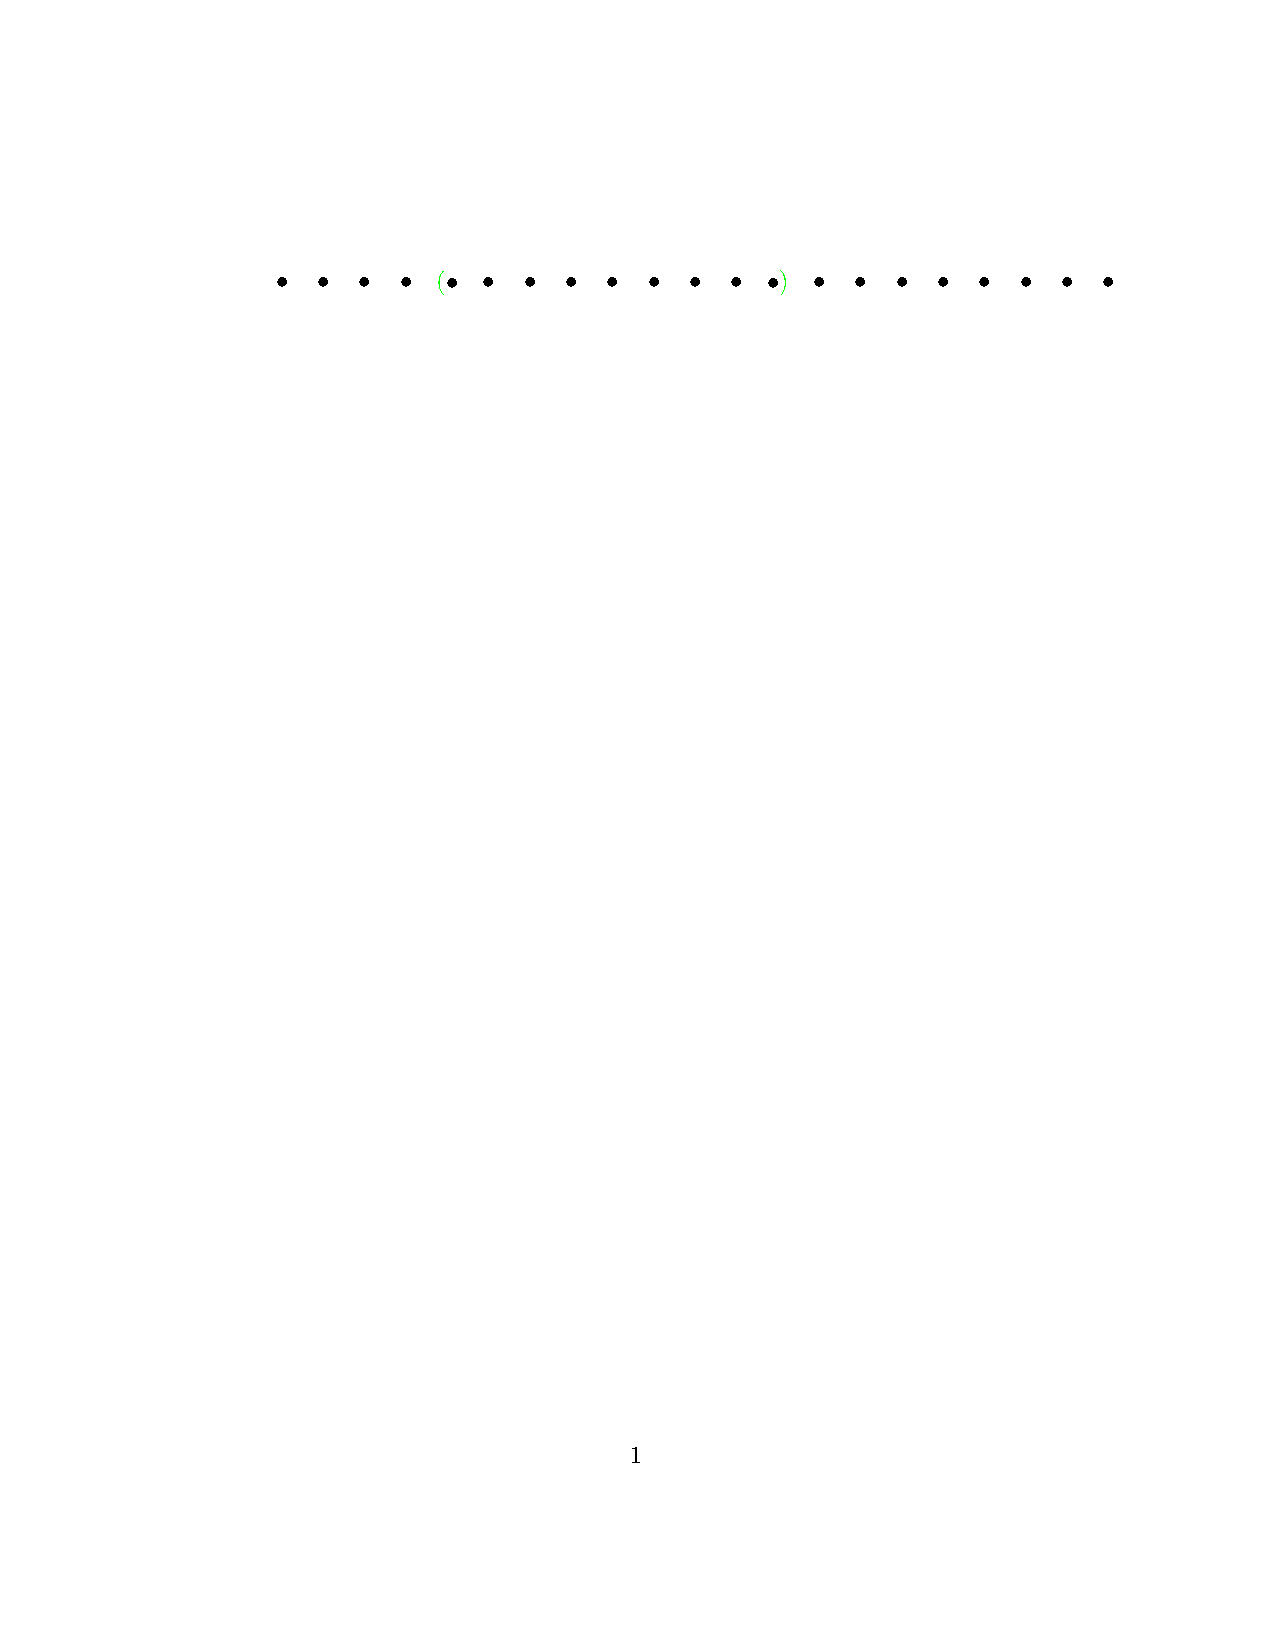
\includegraphics[trim={100 650 30 120},clip,width=\textwidth]{figures/conflictingReq.pdf}
\caption{An example of $n$ points on the real line separated by a small distance $\alpha$. This figure highlights that it is not always possible to satisfy the two requirements from clustering algorithms.}
\label{fig:conflictingReq}
\end{figure}

Hence, different algorithms `focus more' on different aspects of the clustering definition. For example, single-linkage tries to put similar points in the same cluster. However, it may end up having dissimilar points in the same cluster as well. On the other hand, the Lloyd's algorithm tries to separate dis-similar points but may end up separating similar points as well. The basic definition of clustering does not have enough information to resolve this conflict. Thus, we say that the clustering problem is under-specified. The fundamental question that we ask here is that `how do we prefer one clustering algorithm over another?'

We address the problem of under-specificity by incorporating domain knowledge into the clustering problem. The clustering algorithm is allowed to interact with an oracle (or an expert) by asking whether two points should belong to the same or different clusters. The oracle replies either `yes' or `no' to the \textit{same-cluster} query depending upon whether the two points belong to the same or different clusters. In this case, the goal of the clustering algorithm is to recover the clustering which the oracle has in its `mind'.

In the first part of the thesis we simultaneously address the challenges of under-specificity and computational cost. We study the \textit{computational} and \textit{query} complexity of various clustering problems in this framework. Consider the following simple observation. Given any clustering instance, if the algorithm is allowed to make $n^2$ (where $n$ is the size of the dataset) queries to the same-cluster oracle then recovering the true or target clustering is trivial. In this dissertation, one of the important questions that we examine is the following. {Is it possible to efficiently solve (in polyniomial time) an otherwise intractable clustering problem while making a `small' number of same-cluster queries to the oracle?}  

Now, we discuss the third challenge; namely the issue of \textit{noise-robustness} of clustering algorithms. The basic definition of clustering says that the goal is to partition a dataset into clusters such that similar points share a cluster while dissimlar points are separated into different clusters. This definition makes sense when the given dataset has a cohesive structure. That is, the dataset can be partitioned into groups or clusters which have some inter-cluster separation. However, real-world datasets, on top of this structure, have a significant subset of points which are unstructured. The addition of these \textit{noisy} points makes it difficult for the clustering algorithm to detect the structure of remaining points. The precise definition of `unstructuredness' or noisy points varies depending upon the structure that the clustering algorithm is trying to detect. In this dissertation, we consider two definitions of noise and develop efficient noise-robust clustering algorithms in each case.

We address all the challenges of clustering under a formal framework. The goal is to have a framework which can be mathematically analyzed and is also relevant to practitioners. Obviously, the exact framework varies depending upon the clustering problem we are considering. To analyze these issues in a formal framework, we will be mostly relying on mathematical theorems and proofs. But in some cases (where applicable), we have also complemented our results with experiments and simulations. 

\section{Our Contributions} 
As we alluded to before, our contributions can be divided into two categories. One is dealing with under-specificity and the second related to noise robustness of clustering algorithms. In this next sub-sections, we go into more details of each of these and outline our  objectives and contributions made. 

\subsection{Under-specificity}
The first main contribution is to develop a formal framework to incorporate domain knowledge into the clustering problem. We introduce a semi-supervised clustering framework. The learner is allowed to interact with a domain expert (or an oracle) by asking whether two data instances belong to the same  or different cluster (same-cluster query). The oracle has a target clustering in its mind and responds by answering either `yes' or `no' (depending upon whether the two points belong to the same or different clusters according to the target clustering). We assume that the oracle is perfect and has complete knowledge of the ground truth clustering. Hence, given any pair of points it always gives the correct response. We consider two clustering problems under this framework.

\subsubsection*{Clustering with advice ($k$-means)}
We consider a setting where the oracle conforms to a center-based clustering with a notion of margin. That is, the target clustering has the following property.  Every cluster-center is `more' closer ($\gamma$-times closer) to points in its own cluster than to points in a different cluster. Larger values of $\gamma$ imply greater separation between different clusters. 

Under this framework, we study the query and computational complexity of recovering the target clustering. We provide an algorithm which runs in $O\big(kn\log n)$ time and makes $O\big(k\log n + k^2 \log k)$ same-cluster queries to the oracle and succeeds in recovering the oracle's clustering with high probability. Here $n$ is the size of the dataset and $k$ is the number of clusters.

We also consider the case when the oracle conforms to the optimal $k$-means clustering under $\gamma$-margin. Then, our query-based algorithm can find the optimal solution in polynomial time. Interestingly, we prove that even when the optimal $k$-means clustering satisfies margin conditions, without queries, finding that solution is NP-hard. Thus having access to relatively few oracle queries can allow efficient solutions to otherwise intractable problems.

\subsubsection*{Correlation clustering with advice}
We consider the problem of correlation clustering under the semi-supervised clustering framework. Correlation clustering is very useful for modelling the record de-duplication problem; the task of detecting multiple records that correspond to the same real-world entity in a database. Here the goal is to put records corresponding to the same physical entity in the same cluster and putting records corresponding to different physical entities into different clusters.

Formally, given a complete graph $G$ with the edges labelled $0$ and $1$, the goal of correlation clustering is to find a clustering that minimizes the number of $0$ edges within a cluster plus the number of $1$ edges across different clusters. In other words, the goal is to find a clustering which minimizes the \textit{correlation loss} w.r.t the graph $G$. \\

\noindent\textbf{\small Promise correlation clustering}\\
The optimal clustering $C^*$ can also be viewed as a complete graph $G^*$ (unknown to the clustering algorithm) with edges corresponding to points in the same cluster being labelled $1$ and other edges being labelled $0$. If it is known that the edge difference between $G$ and $G^*$ is zero, then finding $C^*$ is easy (find the connected components of $G$). We consider a variant of this problem where it is promised that the edge difference between $G$ and the unknown $G^*$ is ``small". The goal is to find the clustering which minimizes the correlation loss w.r.t $G$.

We now wish to analyze the computational and query complexity of the promise correlation clustering (PCC) problem. We prove that the promise version is still NP-hard. Rather surprisingly, we further prove that even with access to a same-cluster oracle, the promise version is intractable as long as the number queries to the oracle is $o(n)$ (the proof assumes the Exponential Time Hypothesis; $n$ is the number of vertices). \\

\noindent\textbf{\small Restricted correlation clustering}\\
Given these negative results, we consider a restricted version of correlation clustering. First observe that in the standard version, the goal is to find a clustering over the class of all possible clusterings of the dataset. Here, we restrict ourselves to a given class $\mc F$ of clusterings. Another difference is that we want to minimize the correlation loss w.r.t the unknown target clustering $C^*$ rather than a graph $G$. 

We now wish to analyze the query and computational complexity of this problem. We offer an algorithmic approach (using same-cluster queries) and prove that the query complexity is upper bounded by a term that depends only on the $\vcdim(\mc F)$ and is independent of the dataset size. We also provide computationally efficient algorithms for a few common classes of clusterings. 
 
\subsection{Noise-robustness}
We now describe our framework to address the issue of noise in clustering algorithms. We are given a dataset $X$ which is made up of two parts. The first is the structured or clusterable component $S$. Mathematically, this is captured by introducing notions of `clusterability of data'. Intuitively, these notions say that the set $S$ is composed of $k$ different clusters and the clusters are `well-separated' from each other. In this thesis, we consider two such notions, center-proximity and center-separation. Each of them formalize the idea of well-separatedness in a different way. The second component of the dataset is the noisy or unstructured part $N$. The clustering algorithm receives $X$ as its input. It does not have any knowledge about $S$ (or its substructure) or $N$. The goal is to partition $X$ into components so that the structure of $S$ is \textit{preserved}. Any algorithm which achieves this goal is said to be noise-robust. 

\subsubsection*{Detecting cluster structure in the presence of sparse noise}
We consider the problem of detecting the structure of $S$ when the noisy part $N$ is sparse. That is, the only restriction about the noisy part of the data is that it does not create significantly large clusters. We introduce efficient algorithms that discover and cluster every subset $S$ of the data with the following property. $S$ has a meaningful structure (as captured by a notion of clusterability) and its complement is structureless or sparse. We say that our algorithm is robust to sparse noise. Notably, the success of our algorithms do not depend on any upper bound on the fraction of noisy data. We complement our results by showing that when either the notions of structure or the noise requirements are relaxed, no such results are possible.

\subsubsection*{Detecting cluster structure in the presence of outliers}
We propose a generic regularization-based method that transforms any center-based clustering objective into a noise-robust one. We use our procedure to obtain regularized versions of two common clustering algorithms based on the $k$-means objective function. We prove that these regularized algorithms are robust to outliers (under clusterability assumptions and mildness properties of the noisy points).

\section{Reading the thesis}
This dissertation is composed of two components. The first addresses the problem of under-specificity in clustering and is covered in Chapters \ref{chapter:activeClustering} and \ref{chapter:deduplication}. The second part is about the issue of noise-robustness of clustering algorithms and is covered in Chapters \ref{chapter:clusteringNoise} and \ref{chapter:optimizationClustering}. The two parts are independent of one another and the reader can start with whichever one he/she is more interested in. 

We have ensured that each chapter is self-contained. Note that the thesis does not have a dedicated chapter on related work or on notation/preliminaries. Rather these are included in the relevant chapters. Some of the missing proofs can be found in appendices at the end of the corresponding chapters.

\section{Technical background}
Some of the proofs in the thesis use the following classical results from learning theory literature. Readers who are unfamiliar with result can also refer to the standard texts on this subject, for example, \cite{shalev2014understanding}.
 

\subsection{Learning theory results}
\begin{theorem}[Vapnik and Chervonenkis \cite{vapnik2015uniform}]
\label{thm:vceapprox}
Let $X$ be a domain set and $D$ a probability distribution over $X$. Let $H$ be a class of subsets of $X$ of finite VC-dimension $d$. Let $\epsilon, \delta \in (0,1)$. Let $S \subseteq X$ be picked i.i.d according to $D$ of size $m$. If $m > \frac{c}{\epsilon^2}(d\log \frac{d}{\epsilon}+\log\frac{1}{\delta})$, then  with probability $1-\delta$ over the choice of $S$, we have that $\forall h \in H$
$$\bigg|\frac{|h\cap S|}{|S|} - P(h)\bigg| < \epsilon$$
\end{theorem}

\begin{theorem}[Fundamental theorem of learning \cite{blumer1989learnability}] 
\label{thm:uniformConvergence}
Here, we state the theorem as in the book \cite{shalev2014understanding}. Let $H$ be a class of functions $h:\mc X \rightarrow \{0, 1\}$ of finite VC-Dimension, that is $\vcdim(H) = d < \infty$. Let $D$ be a probability distribution over $X$ and $h^*$ be some unknown target function. Given $\epsilon, \delta \in (0, 1)$. Let $err_D$ be the $\{0, 1\}$-loss function $err: H \rightarrow [0, 1]$. That is $err_D(h) = \underset{x \in D}{\mb P}[h(x) \neq h^*(x)]$. Sample a set $S = \{(x_1, y_1), \ldots, (x_m, y_m)\}$ according to the distribution $D$. Define $err_S(h) = \sum_{i=1}^{m} \frac{\mb 1_{[h(x_i) \neq h^*(x_i)]}}{m}$. If $m \ge a\frac{d + \log (1/\delta)}{\epsilon^2}$, then with probability at least $1-\delta$ over the choice of $S$, we have that for all $h \in H$
$$|err_D(h) - err_S(h)| \le \epsilon$$
where $a$ is an absolute global constant. 
\end{theorem}

\subsection{Concentration inequalities}
Some of the proofs use the following concentration inequalities. 
\label{appendixsection:conIneq}
\begin{theorem}[Sum of geometric random variables \cite{brown2011wasted}]
\label{thm:geometricRV}
Let $X = X_1 + \ldots + X_n$ be $n$ geometrically distributed random variables such that $\mb E[X_i] = \mu$. Then 
$$\mb P[X > (1+\nu)n\mu] \le \exp\bigg(\frac{-\nu^2\mu n}{2(1+\nu)}\bigg)$$
\end{theorem}   

\begin{theorem}[Generalized Hoeffding's Inequality (e.g., \cite{ashtiani2015dimension})]
\label{thm:genHoeff}
Let $X_1, \ldots. X_n$ be i.i.d random vectors in some Hilbert space such that for all $i$, $\|X_i\|_2 \le R$ and $E[X_i] = \mu$. If $n > c\frac{\log(1/\delta)}{\epsilon^2}$, then with probability at least $1-\delta$, we have that
$$\Big\|\mu - \frac{1}{n}\sum X_i\Big\|_2^2 \le R^2\epsilon$$ 
\end{theorem}

\begin{theorem}[Multiplicative Chernoff bound \cite{mitzenmacher2005probability}]
\label{thm:chernoff}
Let\\ $X_1, \ldots, X_n$ be i.i.d random variables in $\{0, 1\}$ such that $\mu = E[X_i]$. Let $X = \frac{\sum X_i}{n}$. Then for any $0 < \epsilon < 1$
$$P\big[ \enspace X > (1+\epsilon) \mu\enspace\big] \enspace\le\enspace \exp\bigg(\frac{-\epsilon^2\mu n}{3}\bigg)$$
\end{theorem}

\begin{theorem}[Multiplicative Chernoff bound \cite{mitzenmacher2005probability}]
\label{thm:chernoff2}
Let\\ $X_1, \ldots, X_n$ be i.i.d random variables in $\{0, 1\}$ such that $\mu = E[X_i]$. Let $X = \frac{\sum X_i}{n}$. Then for any $0 < \epsilon < 1$
$$P\big[ \enspace X < (1-\epsilon) \mu\enspace\big] \enspace\le\enspace \exp\bigg(\frac{-\epsilon^2\mu n}{2}\bigg)$$
\end{theorem}


\ifdefined\COMPLETE
\else
\end{document}
\fi






























